\documentclass{article}

\usepackage[left=.75in, right=.75in, top=.75in, bottom=1in]{geometry}
\usepackage{titling}
\usepackage{graphicx}
\usepackage{array}
\usepackage{parskip} 
\usepackage{amsmath}
\usepackage{enumitem}
\usepackage{fancyhdr}

\renewcommand{\arraystretch}{1.5}
\renewcommand{\footrulewidth}{0.4pt}
 
\date{} % This will remove the date

\begin{document}

    \pagestyle{fancy}
    \headheight=10pt
    \fancyhead[C]{\Large\textbf{Math 330} \\ \textbf{Project 1 / Ch 2.2}}
    \fancyhead[L]{\textbf{Name: Larosh Shaikh} \\ \textbf{Date: 12/23/2024}}
    \fancyhead[R]{\textbf{Dr. Andrew Hofstrand} \\ \textbf{Due Date: 12/30/2024}}
    \fancyfoot[C]{\thepage}
    
   
    \textbf{Problem 2.2.1:} Tangent Lines 
    \begin{enumerate}[label=\textbf{\alph*)}]
    \item First, plot the function, $f(x) = ln(x)$, in blue, on the interval $-1 \leq x \leq 6$ and $-2 \leq y \leq 3$. \\
    \item Now find the tangent lines of $f(x)$, using D[], at the points $x = 1$ and $x = e$. Plot the tangent lines in dashed-red and dashed-gray, respectively, on the same domain and range as above.
    \item Plot the two points above on $f(x)$ where you evaluated the tangent lines in black.
    \item Now overlay each of the plots you made above on a single graph. Make sure you can see everything you plotted.
    \end{enumerate}

    \textbf{Problem 2.2.2:} Integrating a discontinuous function 
    \begin{enumerate}[label=\textbf{\alph*)}]
        \item The so-called Heaviside piece-wise function is defined as follows:
        \begin{equation*}
            H(x) = \begin{cases}
                0 & x < 0 \\
                1 & x \geq 0
            \end{cases}
        \end{equation*}
        Plot this function $G(x)= 2H(x)-1$
        \item Now find the indefinite integral of G(x), using Integrate[] and Piecewise[], and plot the resulting function.
        \item Integrate the function you found above another time.
        \item Plot all three functions above, including G(x), on a single graph for $-2 \leq x$, $y \leq 2$ in different colors.
        \item What do you notice about the continuity and smoothness of the indefinite integrals as you keep integrating G(x)? Conversely, what happens when you go backwards and differentiate each expression?
    \end{enumerate}
    
    \vfill
    \newpage

    \headheight=10pt
    \textbf{Solution 2.2.1:} Tangent Lines \\
    \textbf{a)} In order to plot the function, $f(x) = ln(x)$, we first need to define the function. We can do this by using the following code: \\
    \begin{verbatim}
        f[x_] := Log[x]
    \end{verbatim}
    Now that we have defined the function, we can plot it using the following code: \\
    \begin{verbatim}
        Plot[f[x], {x, -1, 6}, PlotRange -> {{-1, 6}, {-2, 3}}]
    \end{verbatim}
    The resulting plot is shown below: \\
    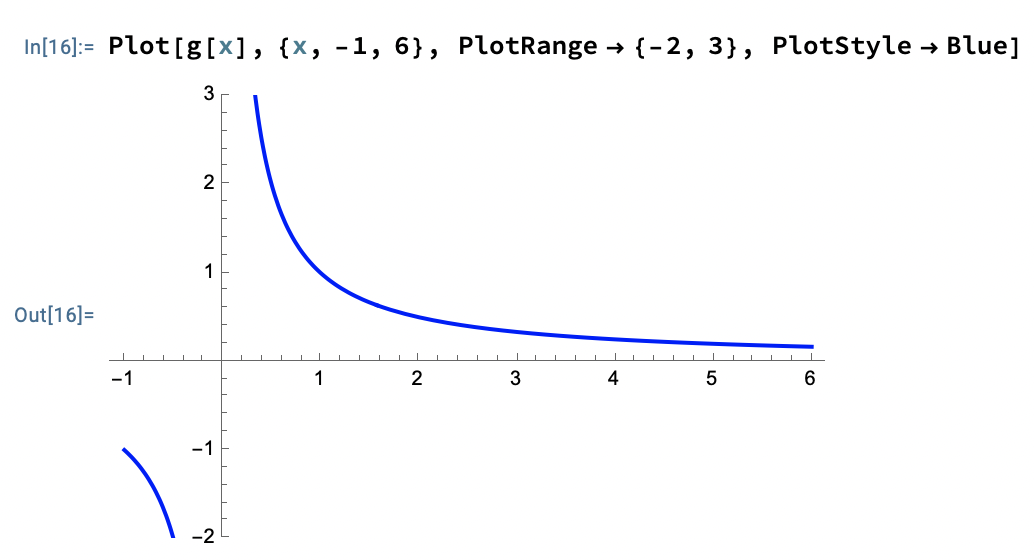
\includegraphics[scale=0.5]{2.2.1a.png} \\

    \textbf{b)} In order to find the tangent lines of $f(x)$, using D[], at the points $x = 1$ and $x = e$, we can do some math ourselves. We know that the derivative of $f(x)$ is $\frac{1}{x}$. We also know that the equation of a line is $y-y_1 = m(x-x_1)$. We can use this information to find the tangent lines of $f(x)$ at the points $x = 1$ and $x = e$. \\

    \begin{equation*}
        \begin{split}
            y-y_1 &= m(x-x_1) \\
            y-0 &= \frac{1}{1}(x-1) \\
            y &= x-1
        \end{split}
    \end{equation*}

    \begin{equation*}
        \begin{split}
            y-y_1 &= m(x-x_1) \\
            y-1 &= \frac{1}{e}(x-e) \\
            y &= \frac{x}{e}
        \end{split}
    \end{equation*}

   We can represent these new functions in Mathematica using the following code: \\
    \begin{verbatim}
          g[x_] := x - 1
          h[x_] := x/e
    \end{verbatim}
    
    Now that we have defined the functions, we can plot them individually using the following code: \\
    \begin{verbatim}
        Plot[g[x], {x, -1, 6}, PlotRange -> {-1, 6}, 
        PlotStyle -> {Red, Dashed}]
        Plot[h[x], {x, -1, 6}, PlotRange -> {-1, 6}, 
        PlotStyle -> {Grey, Dashed}]
    \end{verbatim}

    The resulting plots are shown below: \\
    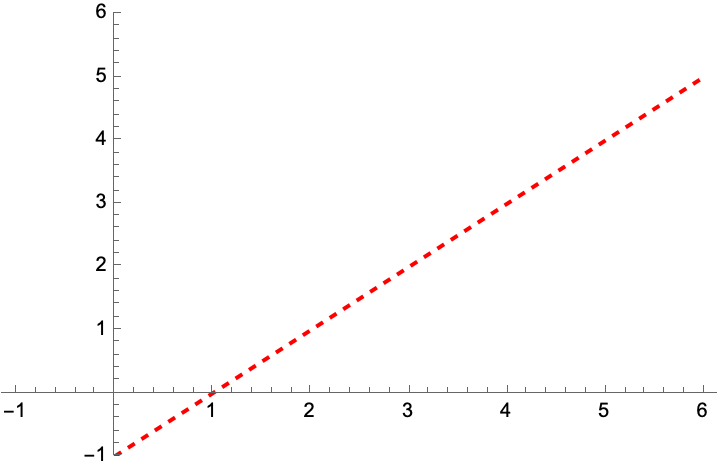
\includegraphics[scale=0.5]{2.2.1b.png} \\
    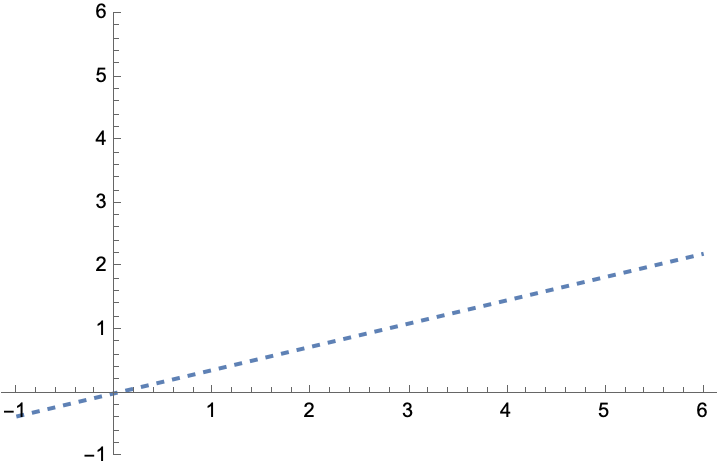
\includegraphics[scale=0.5]{2.2.1b2.png} \\

    \textbf{c)} Now we just want to plot the two points where I evaulated the lines in black. This is achieveable by: \\
    \begin{verbatim}
        Show[Plot[f[x], {x, -1, 6}, PlotRange -> {{-1, 6}, {-2, 3}}], 
        Graphics[{PointSize[Large], Point[{1, 0}], Point[{E, Log[E]}]}]]
    \end{verbatim}
    The resulting plot is shown below: \\   
    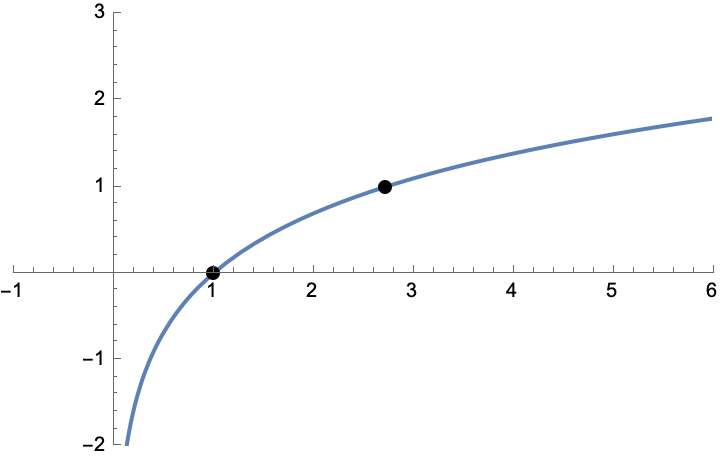
\includegraphics[scale=0.5]{2.2.1c.png} \\


    \textbf{d)} Now we just want to overlay each of the plots we made above on a single graph. This is achieveable by: \\
    \begin{verbatim}
        Show[Plot[f[x], {x, -1, 6}, PlotRange -> {{-1, 6}, {-2, 3}}], 
        Graphics[{PointSize[Large], Point[{1, 0}], Point[{E, Log[E]}]}], 
        Plot[g[x], {x, -1, 6}, PlotRange -> {-1, 6}, 
        PlotStyle -> {Red, Dashed}], 
        Plot[h[x], {x, -1, 6}, PlotRange -> {-1, 6}, 
        PlotStyle -> {Grey, Dashed}]]
    \end{verbatim}
    \vfill 
    \newpage
    The resulting plot is shown below: \\
    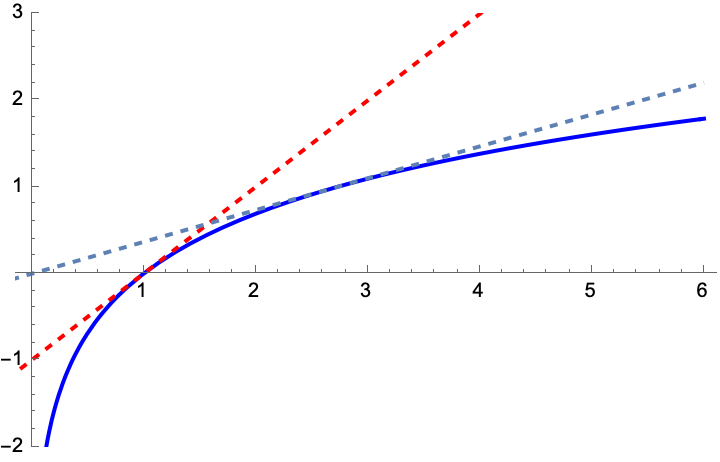
\includegraphics[scale=0.5]{2.2.1d.png} \\

    Alternatively, we could use python to plot these points using the matplotlib library. We can do this by using the following code: \\
    \begin{verbatim}
        import matplotlib.pyplot as plt
        import numpy as np
        
        x = np.linspace(-1, 6, 100)
        y = np.log(x)
        plt.plot(x, y)
        plt.axhline(0, color='black',linewidth=0.5)
        plt.axvline(0, color='black',linewidth=0.5)
        plt.xlim(-1, 6)
        plt.ylim(-2, 3)
        plt.scatter(1, 0, color='black')
        plt.scatter(np.exp(1), np.log(np.exp(1)), color='black')
        y = x - 1
        plt.plot(x, y, color='red', linestyle='dashed')
        y = x/np.exp(1)
        plt.plot(x, y, color='grey', linestyle='dashed')
        plt.show()
    \end{verbatim}
    \vfill
    \newpage
    The resulting plot is shown below: \\
    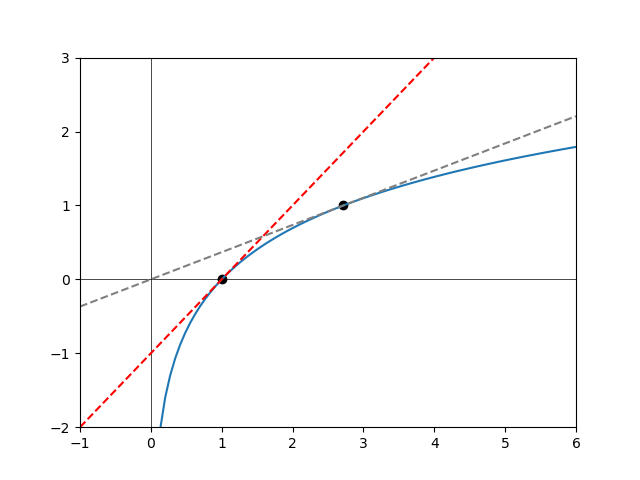
\includegraphics[scale=0.5]{2.2.1d_py.png} \\
   
    \textbf{2.2.1 Notes:} 
    \begin{itemize}
        \item The python code is much more verbose than the Mathematica code. This is because python is a general purpose programming language, while Mathematica is a language specifically designed for mathematical purposes.
        \item The python code is also much more difficult to read than the Mathematica code. 
        \item A syntaxical note, In Mathematica you may notice the usage of $F[x\_]$ versus $F[x]$, this is to notate the input arguments. 
        \item Another syntaxical note, In Mathematica, you may notice we redfine plot range and the values for which x is plotted twice, {x,-1,6} and inside PlotRange. 
        This is because PlotRange is a function that takes in a list of two values, the first being the x range and the second being the y range, but also because PlotRange is defined as where you'd like a plot to extend whereas the x values in the former define where Mathematica evaluates the function. 
        \item There is a rather distinct difference between $e$ and $E$ between versions, please be mindful.
    \end{itemize}

    \vfill
   \newpage
   \headheight=10pt

    \textbf{Solution 2.2.2:} Integrating a discontinuous function \\ 
    \textbf{a)} In order to plot the function, $G(x)= 2H(x)-1$, we first need to define the function. We can do this by using the following code: \\
    \begin{verbatim}
        H[x_] := Piecewise[{{0, x < 0}, {1, x >= 0}}]
        G[x_] := 2*H[x] - 1
    \end{verbatim}
    Now that we have defined the function, we can plot it using the following code: \\
    \begin{verbatim}
        Plot[H[x], {x, -2, 2}, PlotRange -> {{-2, 2}, {-2, 2}}]
        Plot[G[x], {x, -2, 2}, PlotRange -> {{-2, 2}, {-2, 2}}]
    \end{verbatim}
    The resulting plots are shown below: \\
    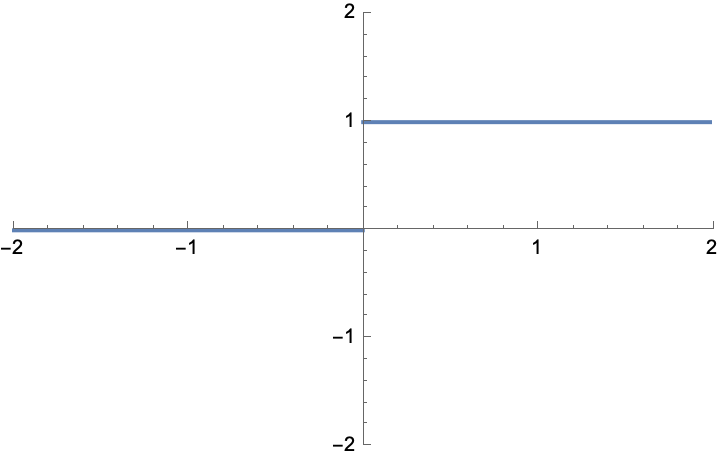
\includegraphics[scale=0.5]{2.2.2a.png} \\
    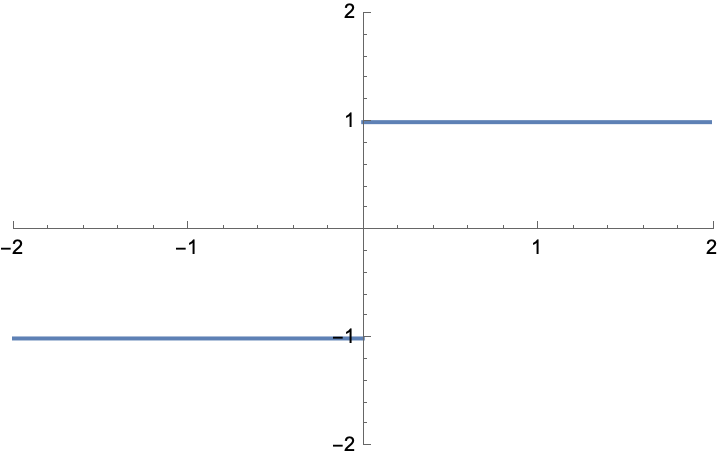
\includegraphics[scale=0.5]{2.2.2a2.png} \\

    \textbf{b)} In order to find the indefinite integral of $G(x)$, we can use Integrate[] and Piecewise[]. We can do this by using the following code: \\
    \begin{verbatim}
        Int1[x_] = Integrate[G[x], x]
    \end{verbatim}
    Integrating a piecewise function in Mathematica proves to be very simple. However, integrating a piecewise function by hand is a bit more difficult. We can do this by using the following steps: \\
    \begin{equation*}
        \begin{split}
            G(x) &= 2H(x)-1 \\
            &= 2(0)-1 \text{ for } x < 0 \\
            &= -1 \\
            &= 2(1)-1 \text{ for } x \geq 0 \\
            &= 1 \\
            &= \int G(x) dx \\
            &= \int -1 dx \text{ and}  \int 1 dx \\
        G(x)&= -x \text{ for } x < 0 \\
        G(x)&= x \text{ for } x \geq 0 \\
        \end{split}
    \end{equation*}
    Now that we have found the indefinite integral of $G(x)$, we can plot it using the following code: \\
    \begin{verbatim}
        Plot[Piecewise[{{-x, x <= 0}}, x], {x, -2, 2}]
    \end{verbatim}
    The resulting plots are shown below: \\
    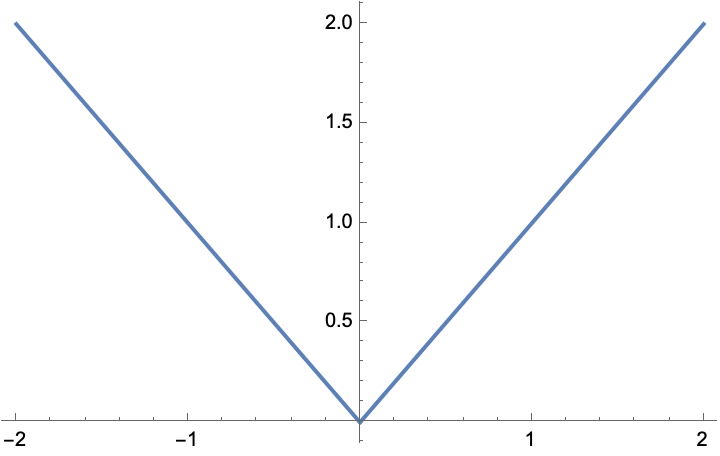
\includegraphics[scale=0.5]{2.2.2b.png} \\

    \textbf{c)} In order to integrate the function we found above another time, we can use the following code: \\
    \begin{verbatim}
        Int2[x_] = Integrate[Int1[x], x]
    \end{verbatim}
    Now that we have found the second integral of $G(x)$, we can plot it using the following code: \\
    \begin{verbatim}
        Plot[Piecewise[{{-(x^2/2), x <= 0}}, x^2/2], {x, -2, 2}]
    \end{verbatim}
    The resulting plots are shown below: \\
    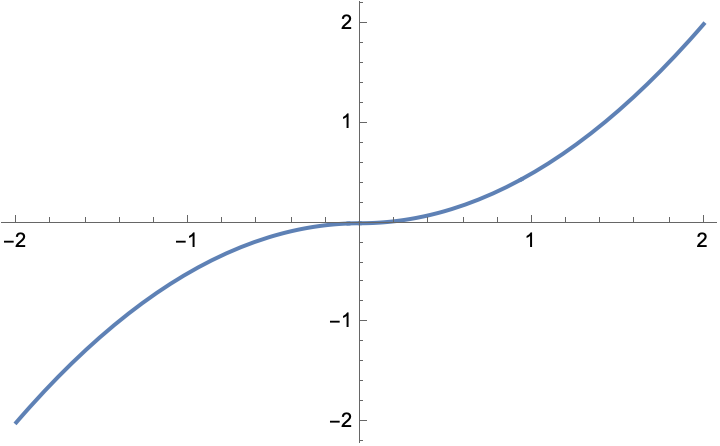
\includegraphics[scale=0.5]{2.2.2c.png} \\

    \textbf{d)} In order to plot all three functions above, including $G(x)$, on a single graph for $-2 \leq x$, $y \leq 2$ in different colors, we can use the following code: \\
    \begin{verbatim}
        Plot[{Piecewise[{{0, x < 0}, {1, x >= 0}}], 
        Piecewise[{{-x, x <= 0}}, x], 
        Piecewise[{{-(x^2/2), x <= 0}}, x^2/2]}, {x, -2, 2}, 
        PlotRange -> {{-2, 2}, {-2, 2}}]
    \end{verbatim}

    The resulting plot is shown below: \\
    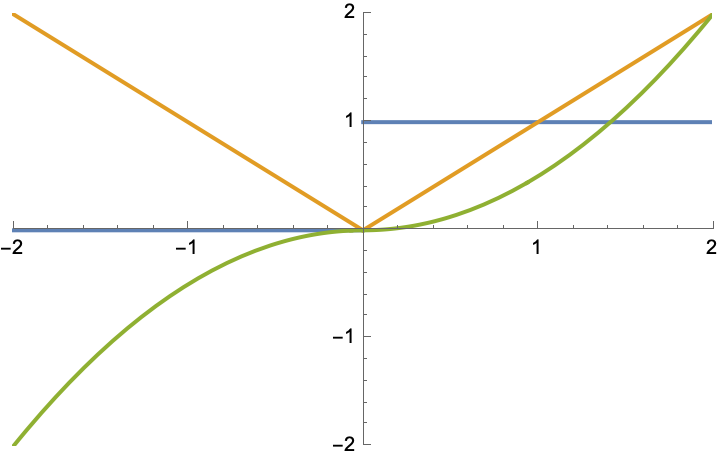
\includegraphics[scale=0.5]{2.2.2d.png} \\

    \textbf{e)} As we keep integrating $G(x)$, we notice that the function becomes more and more smooth. Conversely, as we keep differentiating $G(x)$, we notice that the function becomes more and more discontinuous. \\

    Alternatively, we could use python to plot these points using the matplotlib library. We can do this by using the following code: \\
    \begin{verbatim}
        import matplotlib.pyplot as plt
        import numpy as np
                
        x = np.linspace(-2, 2, 100)
        y = np.piecewise(x, [x < 0, x >= 0], [0, 1])
        plt.plot(x, y)
        y = np.piecewise(x, [x < 0, x >= 0], [lambda x: -x, lambda x: x])
        plt.plot(x, y)
        y = np.piecewise(x, [x < 0, x >= 0], [lambda x: -x**2/2, lambda x: x**2/2])
        plt.plot(x, y)
        plt.axhline(0, color='black',linewidth=0.5)
        plt.axvline(0, color='black',linewidth=0.5)
        plt.xlim(-2, 2)
        plt.ylim(-2, 2)
        plt.show()
    \end{verbatim}
    \vfill
    \newpage 
    \headheight=10pt
    The resulting plot is shown below: \\
    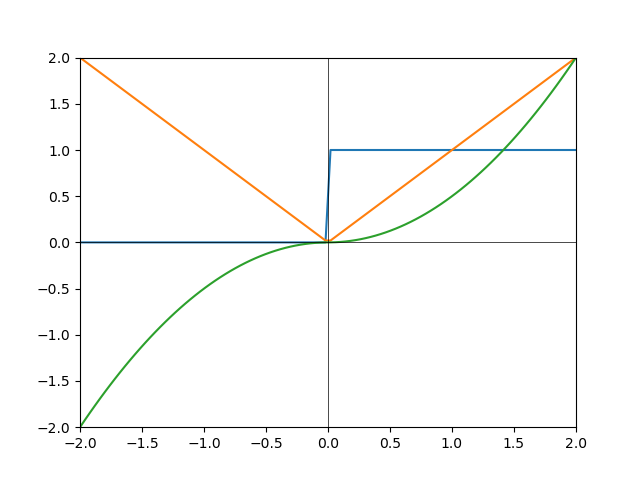
\includegraphics[scale=0.5]{2.2.2d_py.png} \\

    \textbf{2.2.2 Notes:} 
    \begin{itemize}
        \item We name the integration functions so that we can refer to them later on. I have yet to come up with a more solid naming mechanism, but for now this will have to do.
        \item You'll notice we do not have to distinguish line colors inside our plot, this is done when plotting 3 seperate functions. Alternatively we could create 3 plots, and use Show[] to combine them, but this is not necessary.
    \end{itemize}
    
\end{document}
